
Highway-env es una biblioteca de código abierto que proporciona una colección de entornos
de conducción para aprendizaje por refuerzo, desarrollada por Leurent \cite{highway-env}.
Esta biblioteca implementa diversos escenarios vehiculares, incluyendo fusión en autopistas,
intersecciones y particularmente relevante para este trabajo, el entorno de estacionamiento.
La Figura~\ref{fig:highway-env-scenarios} ilustra algunos de los entornos disponibles en esta biblioteca.

\begin{figure}[!ht]
    \centering
    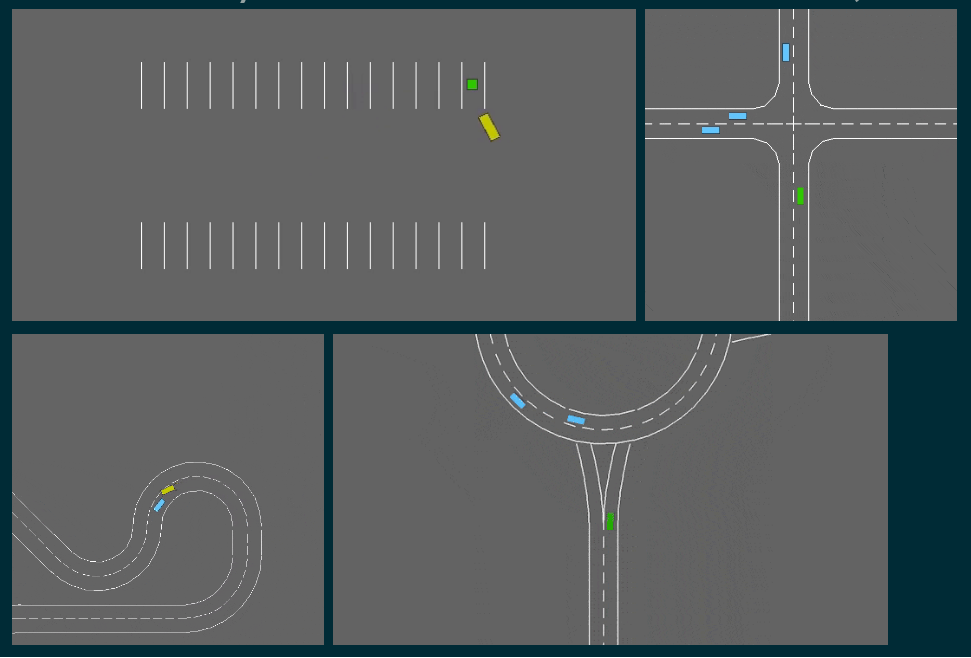
\includegraphics[width=0.85\textwidth]{img/2-mt/higthway-env.png}
    \caption{Ejemplos de entornos disponibles en Highway-env: estacionamiento, intersecciones, fusión en autopistas y rotondas.}
    \label{fig:highway-env-scenarios}
\end{figure}

\subsection{Entorno de estacionamiento en Highway-env}\label{subsec:highway-env-theory}

El entorno \texttt{parking-v0} de Highway-env modela la tarea de estacionamiento como un
problema de aprendizaje por refuerzo con las siguientes características:


\textbf{Espacio de observación}: El estado se representa como un vector que incluye
la posición, velocidad y orientación del vehículo, así como información sobre
obstáculos y el objetivo. La observación por defecto es:
\begin{equation}
    \mathbf{s} = [x, y, v_x, v_y, \cos(\theta), \sin(\theta), x_{\text{goal}}, y_{\text{goal}}]
\end{equation}


\textbf{Espacio de acciones}: Utiliza un espacio continuo bidimensional para el control
vehicular: $\mathcal{A} = \text{Box}([-1, -1], [1, 1])$ donde cada acción representa
[aceleración, ángulo de dirección].


\textbf{Función de recompensa}: La recompensa está diseñada para incentivar el progreso
hacia el objetivo mientras penaliza colisiones y maniobras bruscas:
\begin{equation}
    r = r_{\text{objetivo}} + r_{\text{colisión}} + r_{\text{acción}}
\end{equation}

donde cada componente evalúa diferentes aspectos del comportamiento del agente.


\textbf{Simulación física}: El entorno original utiliza un modelo físico simplificado
con cinemática y dinámicas linealizadas, suficiente para el aprendizaje
de políticas pero alejado del realismo de un vehículo real.

\subsection{Ventajas y limitaciones para aplicaciones realistas}

\textbf{Ventajas}:
\begin{itemize}
    \item Interfaz estándar compatible con bibliotecas de RL (Stable-Baselines3, Ray RLLib)
    \item Funciones de recompensa y espacios de acción validados empíricamente
    \item Convergencia probada de algoritmos como PPO, SAC y TD3
    \item Facilidad de uso y documentación extensa
\end{itemize}


\textbf{Limitaciones}:
\begin{itemize}
    \item Observaciones perfectas (sin ruido ni oclusiones)
    \item Física vehicular simplificada
    \item No considera aspectos sensoriales realistas (procesamiento de imágenes)
    \item Entorno visual abstracto alejado de condiciones reales
\end{itemize}


Estas limitaciones motivan la adaptación realizada en este trabajo, donde mantenemos
las fortalezas del framework pero introducimos elementos más realistas a través de
la integración con CARLA y el sistema de visión por computadora desarrollado.
